\chapter{Arkitektur} 
Traffic Control(TC) er delt op ved brug af Client-Server arkitektur og 3-tier modellen. 
\newline
Client-Server arkitekturen er brugt, da alle enheder kommunikerer ind til en central enhed. Dette giver den fordel at alle enheder har adgang til de samme data.
\newline
De 3-tier's i TC kan ses på figur \ref{fig:TierModel}. Det nederste lag er databasen hvor alle data i systemet gemmes. Det midterste lag er business logic, i dette lag ligger den del af koden som behandler data der giver systemet dets funktionalitet. Det øverste lag er presentation, hvilket er det eneste lag brugeren kender og skal forholde sig til. Her bliver alt data vist for brugeren, og brugeren kan tilføje ny data. 
\newline
Fordelen ved 3-tier modellen er at den er skalerbar, der kan nemt tilføjes flere enheder og brugere.
\newline 
Hvis antallet af brugere stiger vil serveren blive belastet. Her giver 3-tier modellen den fordel, at det er nemt at tilføje flere servere i business eller database laget parallelt. 
Dette gøres ved hjælp af en load balancer, der vil kunne tilføje flere webservere i business laget. I database laget ville der skulle laves database replication der gør, at flere database server indeholder det samme data.

\begin{figure}[htbp] % (alternativt [H])
	\centering
	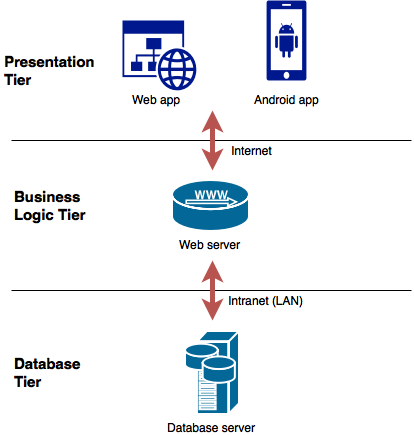
\includegraphics[width=0.6\textwidth]{../Dokumentation/Arkitektur/Tier.png}
	\caption{Tier model for Traffic Control}
	\label{fig:TierModel}
\end{figure}
\clearpage

Både web og Android applikationen er delt op i 3 lag, data access, business logic og presentation. Hvilket giver en god seperation of concern. Der vil fx kunne laves et nyt design, uden der skal ændres i koden for de 2 andre lag. Android applikationen bruger et web API for at tilgå data i databasen, dette betyder at udvikleren for Android applikationen ikke skal kende til opbygningen af databasen. Web applikationen vil også kunne anvende API'et for at tilgå data.
\newline
Sammenspillet mellem de forskellige dele kan ses på figur \ref{fig:OverordnetArkitektur}. Det ses også at notification, har direkte adgang til databasen. Dette skyldes, at notification både indeholder data acces- og business lag. Notification har til ansvar at udsende notifikationer der ligger i kø til at blive send.

\begin{figure}[htbp] % (alternativt [H])
	\centering
	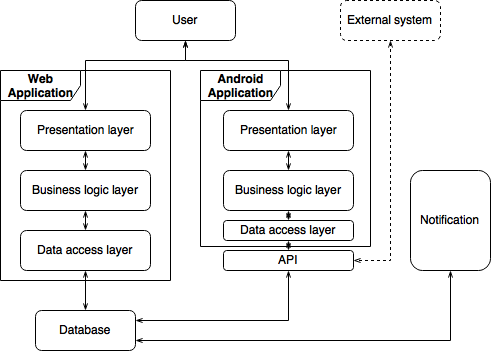
\includegraphics[width=0.8\textwidth]{../Dokumentation/Arkitektur/OverordnetArkitektur.png}
	\caption{Overordnet arkitektur for Traffic Control}
	\label{fig:OverordnetArkitektur}
\end{figure}

\clearpage
